\chapter{Entwicklung}\label{ch:development}

Die Reed-Solomon-Codes wurden 1960 von den amerikanischen Mathematikern Irving S. Reed und Gustave Solomon am Licoln Laboratory des MIT entwickelt.
Sie veröffentlicheten das Paper \textquote{Polynomial codes over certain finite fields}, indem das neu entworfene Fehlerkorrekturverfahren beschrieben wird.
Dabei handelt es sich um Vorwärtskorrektur-Verfahren, welches eigenständig Fehler erkennen und beseitigen kann \cite{wickerReedSolomonCodes1994}.
Durch diese Veröffentlichung wurde eine neue Klasse von \acrlong{ecc}s (\acrshort{ecc}) geschaffen. 
Sie gehört zu der Gruppe der linearen, zyklischen Block-Codes, \dahe zu codierende Daten werden in Wörter der Länge \(n\) geteilt und einzeln weiterverarbeitet \cite{friedrichsKanalcodierung1996}. Ein Ausschnitt der Code-Hierarchie ist in Abbildung \ref{fig:eccHierarchy} dargestellt.

\begin{figure}[h]
	\centering
	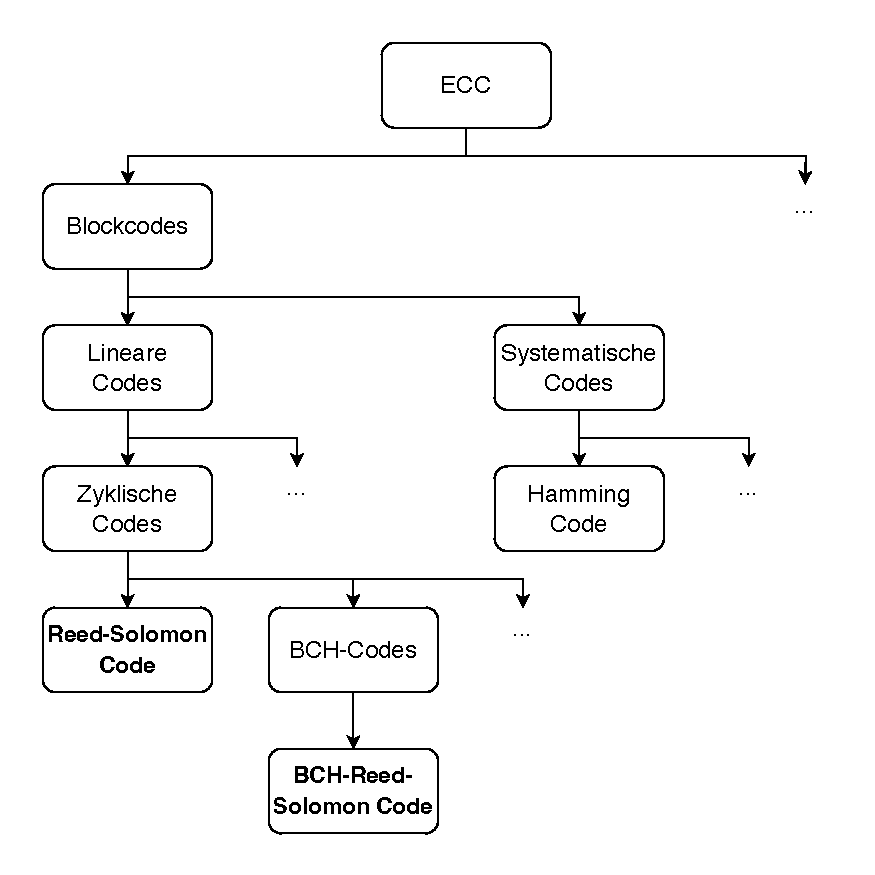
\includegraphics[width=0.9\textwidth]{figures/Codeklassen.drawio.pdf}
	\caption{Ausschnitt der Hierarchie von \acrshort{ecc}}
	\label{fig:eccHierarchy}
\end{figure}

Allerdings war für das Reed-Solomon Verfahren anfangs noch kein effizienter Decodieralgorithmus bekannt, weshalb daran weiter geforscht und weiterentwickelt wurde.
1963 stellte J. J. Stone ein Reed-Solomon-Code vor, der auf dem Schema der auf dem \acrfull{bch} Verfahren basiert \cite{petersonErrorcorrectingCodes1972}.
Dieser Ansatz wird zwar auch als Reed-Solomon-Code bezeichnet, es handelt sich dabei aber um ein weiteres Verfahren, welches seperat vom ursprünglichen Ansatz weiterentwickelt wurde.
Nachdem für die \acrshort{bch}-Codes 1969 ein effizienter Algorithmus, der so genannte Berlekamp-Massey Algorithmus, gefunden wurde, war auch der Einsatz der auf \acrshort{bch} basierende Reed-Solomon-Code in der Praxis verwendbar \cite{berlekampNonbinaryBCHDecoding1968, masseyShiftregisterSynthesisBCH1969}.

Dieses Verfahrens fand zum ersten Mal Anwendung im Jahr 1977 beim Voyager Programm der NASA \cite{wickerReedSolomonCodes1994}. 
Dadurch konnte eine robustere Kommunikation zwischen dem Raumfahrzeug und dem Raumfahrtkontrollzentrum bei einer großen Entfernung zur Erde gewährleistet werden \cite{ludwigVoyagerTelecommunications2002}.
Das erste kommerzielle, an den Endkunden gerichtete Produkt, in dem das Reed-Solomon Verfahren anwendung fand, war 1982 die \acrfull{cd}.

Im Jahr 1986 ermöglichte der Berlekamp-Welch-Algorithmus eine entscheidende Weiterentwicklung. Entwickelt von Elwyn Berlekamp und Lloyd Welch, verbesserte dieser Algorithmus die Effizienz des ursprünglichen Reed-Solomon-Schemas erheblich. Diese Weiterentwicklung förderte die Verbreitung der Reed-Solomon-Codes in verschiedenen Anwendungsbereichen. Eine detailiierte beschreibeung dieser findet sich in Kapitel \ref{ch:application}.

Die kontinuierliche Weiterentwicklung und Anwendung der Reed-Solomon-Codes in verschiedenen Bereichen zeigt die Bedeutung und Vielseitigkeit dieser Fehlerkorrekturverfahren. Um ein tieferes Verständnis der Funktionsweise und der mathematischen Prinzipien hinter diesen Codes zu erlangen, ist es unerlässlich, die theoretischen Grundlagen zu betrachten. Im nächsten Kapitel werden daher die mathematischen Konzepte und Algorithmen erläutert, die den Reed-Solomon-Codes zugrunde liegen.